\fininteract extends formulation in Sec. \ref{sec:task} as a semi-automated ambiguous financial QA corpus built from public filings. Each carries a programmatically verifiable answer, a paired default and intended interpretation produced by an LLM construction pipeline with minimal human annotation and validated by domain experts. Figure~\ref{fig:framework} shows a worked instance and how the benchmark scores an agent's two resolution paths.

\subsection{Design Goals and Principles}
\textbf{Design goals.} \fininteract targets four goals: \textbf{(G1) Representative coverage} to draw real ambiguity from public filings. 
\textbf{(G2) Fine-grained diagnosis} to contain diverse possible readings so that evaluation can localize which clarification ability a model lacks. \textbf{(G3) Low-cost, leak-safe construction} to build and verify the corpus at scale in a semi-automated setting. \textbf{(G4) High, human-validated quality} to validate the instances and judges by domain experts with minimal annotation cost.

\textbf{Design principles.} To satisfy the four goals, we build \fininteract under four principles: \textbf{1): Easy to verify, Ambiguous to resolve} to create programmatically verifiable ground truth using SEC XBRL facts and CNINFO-structured data but the question cannot be correctly resolved without disambiguating context $C$, \textbf{2): No yes/no questions} so that the agent has to deliver a grounded reasoning support, \textbf{3): Includes company name} to ensure no ambiguity in entity, i.e. capitalized proper noun for English and CJK company name for Chinese, and \textbf{4): Answer is not in disambiguating context $C$} so the agent cannot take shortcut by copying directly from the context.  

\subsection{Data Sources}
\label{sec:stats}
We build the instances from official filings. For English instances which take about 80\% of the passage pool, we build them from SEC filings, DocFinQA long-context 10-K/10-Q passages with verified QA pairs and XBRL-derived facts for S\&P~500 and Russell~1000 companies within the financial year of 2024 to 2025. For Chinese instances, we build them from A-share annual reports of SSE~50 and CSI~3000 constituents using CNINFO and akshare structured APIS. We avoid reusing published QA pairs directly to reduce memorization risk, though we do not claim absolute contamination safety. The current evaluation corpus contains 173 instances over 61 companies within 2022 to 2025 filings, labelled with ambiguous taxonomy from Sec. \ref{sec:task}, with detail breakdown in Table~\ref{tab:stats}. Specific details regarding passage counts and difficulty distribution are included in Appendix~\ref{app:construction}.

\begin{table}[t]
\centering
\caption{FinInteract dataset statistics. Disambiguation entropy
$H_0=\log_2 k$ over $k$ plausible interpretations.}
\label{tab:stats}
\small
\resizebox{0.9\columnwidth}{!}{%
\begin{tabular}{lr}
\toprule
Property & Value \\
\midrule
Total instances        & 173 \\
Language (EN / ZH)     & 53 / 120 \\
Source (EDGAR / CSRC-CNINFO / DocFinQA) & 50 / 120 / 3 \\
Filing type (10-K / annual report) & 53 / 120 \\
Unique companies       & 61 \\
Filing years (2022/23/24/25) & 40 / 53 / 58 / 19 \\
\midrule
Primary category: entity\_scope     & 94 \\
\quad metric\_definition        & 63 \\
\quad recognition\_policy       & 9 \\
\quad temporal\_scope           & 7 \\
\quad filing\_vintage           & 0 \\
\# categories (single / two)          & 128 / 45 \\
\midrule
$H_0$ (mean / median / range)   & 2.20 / 2.00 / 1.0--3.6 \\
Mean blind-solve rate (verifier) & 0.7\% \\
\bottomrule
\end{tabular}}
\end{table}

\subsection{Curation}
\label{sec:construction}
We curate each instance from a three-role pipeline, where a \textbf{constructor} agent using GPT-5 generates the full $(Q, C, A)$ triple together with the default and intended interpretations and category label from a filing passage. Specifically, we include category specific instructions to prevent drifting towards categories that are easy to generate. Next, we conduct a \textbf{sanity check} on code level to reject malformed passages instantly without API calls. Lastly, we employ an \textbf{adversarial verifier} to run multiple trial rounds to answer the question $Q$ without disambiguating context $C$ and reject instance where more than two trials produce the intended answer and interpretation simultaneously. Details regarding the prompt, sanity checking codes, output schema and cost are included in Table~\ref{tab:qc}, Appendix~\ref{app:construction} and Appendix~\ref{app:cost}.

\begin{figure*}[t]
\centering
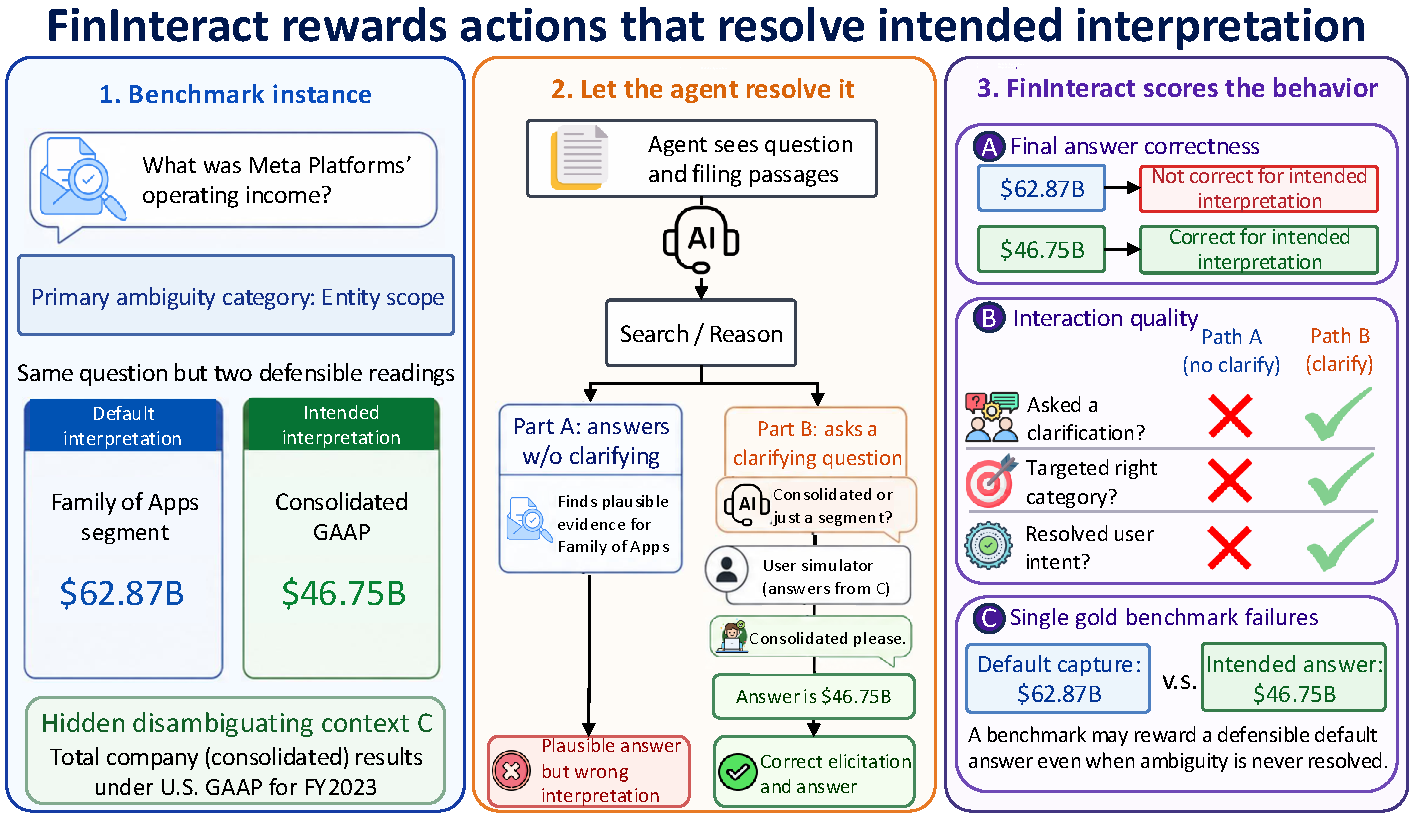
\includegraphics[width=\textwidth]{workflow_plot.pdf}
\caption{\textbf{\fininteract rewards actions that resolve the intended interpretation.}
\textbf{(1)~Benchmark instance:} the question (Meta Platforms' operating income) carries a
primary ambiguity category (entity scope) and two defensible readings, a default (Family of
Apps segment, \$62.87B) and an intended (consolidated GAAP, \$46.75B), separated by a hidden
disambiguating context $C$. \textbf{(2)~Let the agent resolve it:} seeing the question and
filing passages, the agent either answers without clarifying (Part~A, a plausible but wrong
interpretation) or asks a clarifying question that a user simulator answers only from $C$
(Part~B, correct elicitation and answer). \textbf{(3)~\fininteract scores the behavior}
on three signals: final-answer correctness against the intended interpretation, interaction
quality (did the agent ask, target the right category, and resolve the user's intent), and
the single-gold failure a conventional benchmark makes by rewarding the defensible default.}
\label{fig:framework}
\end{figure*}

\subsection{Validation}
\label{sec:humanval}
We employ finance-literate annotators, including Chartered Financial Analyst (CFA) charterholders and licensees from Hong Kong Securities and Futures Commission (SFC), to review instances to check whether 1) question $Q$ is ambiguous and 2) disambiguating context $C$ uniquely identifies the intended reading without stating the answer and 3) both intended and default answers are correct. We record a substantial agreement with an average 0.85 Gwet's AC1~\citep{gwet2008}, indicating strong chance-corrected consensus that, unlike Cohen's $\kappa$, stays reliable under the heavy skew toward ``yes'' labels. The full protocol and annotation details are in Appendix~\ref{app:construction}.

\subsection{Metrics}
\label{sec:metrics}

We deliberately lead with metrics that are standard in the ambiguous-QA and
interactive-retrieval literature (accuracy, calibration, interaction counts),
so that \fininteract is directly comparable to prior benchmarks rather than
self-referential. A single bespoke efficiency score is reported only as a
supplementary diagnostic.

\textbf{Accuracy (\%)} (primary) is the fraction of instances whose final
answer matches the \emph{intended} interpretation, graded by GPT-4o-mini with
financial-domain tolerance ($\pm$1\% numeric, entity/ticker equivalence,
currency normalization; fiscal-year mismatch = wrong). This is the metric on
which models are ranked, mirroring \interactcomp, BrowseComp, and FinanceBench.

\textbf{Default-capture rate (\%)} is the fraction whose final answer instead
matches the \emph{default} interpretation. It measures how often a model
confidently returns the naive reading, and lets us reconstruct what a
conventional single-gold benchmark would have scored (\S\ref{sec:illusion}).

\textbf{Interaction diagnostics} (secondary, descriptive): \emph{IR}
(interaction rate, \% of instances with $\geq 1$ ask), \emph{Round} (mean
turns), and \emph{CategoryHit}, for each interact action GPT-4o-mini classifies
whether the clarifying question targets a true ambiguity category for that instance;
we report CategoryHit@1, AnyCategoryHit, WrongCategoryRate, and GenericAskRate. Because
clarifications are often compound (one question can name an entity, a period, and a metric
at once), we report CategoryHit@1 in two forms: a lenient \emph{touch} form (the question names
any true category) and a strict \emph{central} form (the single most-central category is a true
category). The touch form is validated against human annotators (\S\ref{sec:humanval}). These
metrics characterize \emph{how} a model interacts and do not rank models.

\textbf{Calibration}: 5-bin Expected Calibration Error (ECE) between stated
confidence and correctness, capturing overconfidence on ambiguous queries.

\textbf{\disep (supplementary).} As a single number folding accuracy and
clarification cost together we report the efficiency of \emph{successful}
clarification,
\[
  \text{DisE}^+ = \mathbf{1}[\text{correct}] \times
  \mathbf{1}[n_\text{asks}{>}0] \times \frac{H_0}{n_\text{asks}},
\]
which is positive only when the agent asked at least one question and then
answered correctly, and decreases with redundant asks. We restrict it to the
asked-and-correct case precisely to avoid the perverse incentive of an
all-instances variant, which would award its maximum to a confident
\emph{zero-ask} answer, rewarding the very behavior the benchmark penalizes.
DisE$^+$ is a diagnostic of clarification efficiency, never the ranking metric.
